\documentclass{article}

\usepackage[final]{neurips_2025}

\usepackage[utf8]{inputenc}
\usepackage[T1]{fontenc}
\usepackage{hyperref}
\usepackage{url}
\usepackage{booktabs}
\usepackage{array}
\usepackage{amsmath}
\usepackage{amsfonts}
\usepackage{nicefrac}
\usepackage{microtype}
\usepackage{xcolor}
\usepackage{graphicx}

\definecolor{pass}{HTML}{2E7D32}
\definecolor{fail}{HTML}{C62828}

\title{ARC-AGI-3 Claude Code Harness: Experiment Summary}

\author{
  Sathvik R. \\
  \texttt{sathvik@example.com}
}

\begin{document}

\maketitle

\begin{abstract}
We present an experiment evaluating a Claude Code--based harness for solving ARC-AGI-3 puzzle games.
The harness operates in a single-pass pipeline: Claude reads the game's Python source, analyzes the mechanics, and produces per-level move sequences in one invocation.
We evaluate on 6 games (\texttt{ar25}, \texttt{bp35}, \texttt{cd82}, \texttt{cn04}, \texttt{dc22}, \texttt{ls20}) spanning 41 total levels.
The harness solves \textbf{26 levels} across all games, fully clearing 4 of 6 games: \texttt{ar25} (8/8), \texttt{cd82} (6/6), \texttt{ls20} (7/7), and \texttt{cn04} (5/5).
We analyze failure modes, timing characteristics, and the effect of extended action spaces (clicks, special actions).
\end{abstract}

% ============================================================
\section{Introduction}

This report summarizes an experiment evaluating a Claude Code--based harness for solving ARC-AGI-3 puzzle games.
The harness operates in a single-pass pipeline: Claude Code reads the game's Python source, analyzes the mechanics, and produces per-level move sequences in one invocation.
The experiment was conducted on 6 games of varying complexity from the ARC-AGI-3 benchmark (runs \texttt{20260328\_101645} and \texttt{20260328\_132737}).

% ============================================================
\section{Experimental Setup}

\subsection{Harness Architecture}
The harness (\texttt{harness.py}) orchestrates the following pipeline:
\begin{enumerate}
  \item \textbf{Game loading.} The target game is instantiated locally via \texttt{arcengine}, which provides the game engine, frame rendering, and action execution.
  \item \textbf{Single-pass analysis \& solving.} Claude Code CLI is invoked once in print mode (\texttt{claude -p}) with access to the game's \texttt{source.py}. The prompt asks Claude to analyze the game mechanics and produce a JSON action sequence for \emph{every} level in a single response. This replaces the previous two-phase pipeline (separate analysis + per-level solving).
  \item \textbf{Move parsing.} The harness parses per-level move sequences from the response, looking for \texttt{\#\#\# Level N} headers followed by \texttt{```json} fenced arrays of action IDs. Click actions are encoded as \texttt{[6, x, y]} tuples.
  \item \textbf{Action execution.} Parsed moves are replayed on the local engine. The harness detects level advancement, win, or game-over states to decide whether to proceed.
\end{enumerate}

\subsection{Configuration}
\begin{itemize}
  \item \textbf{Games evaluated:} \texttt{ar25}, \texttt{bp35}, \texttt{cd82}, \texttt{cn04}, \texttt{dc22}, \texttt{ls20}
  \item \textbf{CLI invocation:} \texttt{claude -p --output-format json --dangerously-skip-permissions}
  \item \textbf{Timeout:} 10\,800\,s (3\,h) per game
  \item \textbf{Action space:} $\{1\!=\!\text{UP},\; 2\!=\!\text{DOWN},\; 3\!=\!\text{LEFT},\; 4\!=\!\text{RIGHT},\; 5\!=\!\text{ACTION5},\; 6\!=\!\text{CLICK}(x,y),\; 7\!=\!\text{ACTION7}\}$. Per-game available actions are subset-restricted by \texttt{arcengine}.
  \item \textbf{Single-pass mode:} All reasoning (source analysis + move generation for every level) happens in one Claude Code invocation. No per-level frames are sent.
\end{itemize}

% ============================================================
\section{Results}

\subsection{Aggregate Performance}

\textbf{Total: 26 levels solved out of 41 across 6 games (63\%).}
Table~\ref{tab:summary} summarizes per-game results, using the best run for each game.

\begin{table}[h]
\centering
\caption{Per-game results across all 6 evaluated games.}
\label{tab:summary}
\begin{tabular}{@{}llcccll@{}}
\toprule
\textbf{Game} & \textbf{Levels} & \textbf{Solved} & \textbf{Total Moves} & \textbf{Analysis (s)} & \textbf{Actions} & \textbf{Failure Mode} \\
\midrule
\texttt{ar25} & 8 & \textcolor{pass}{\textbf{8/8}} & 253 & 2103.6 & 1--7 & --- (all solved) \\
\texttt{cd82} & 6 & \textcolor{pass}{\textbf{6/6}} & 76  & 1745.2 & 1--7 + clicks & --- (all solved) \\
\texttt{ls20} & 7 & \textcolor{pass}{\textbf{7/7}} & 311 & 1765.8 & 1--4 & --- (all solved) \\
\texttt{cn04} & 5 & \textcolor{pass}{\textbf{5/5}} & 108 & 654.7  & --- & --- (all solved) \\
\texttt{bp35} & 9 & 0 & 0   & 3600.1 & 3,4,6,7 & L1 timeout / no moves \\
\texttt{dc22} & 6 & 0 & 0   & 2700.0 & --- & L1 no moves parsed \\
\midrule
\textbf{Total} & \textbf{41} & \textbf{26} & \textbf{748} & & & \\
\bottomrule
\end{tabular}
\end{table}

% ============================================================
\section{Plots}

\begin{figure}[h]
\centering
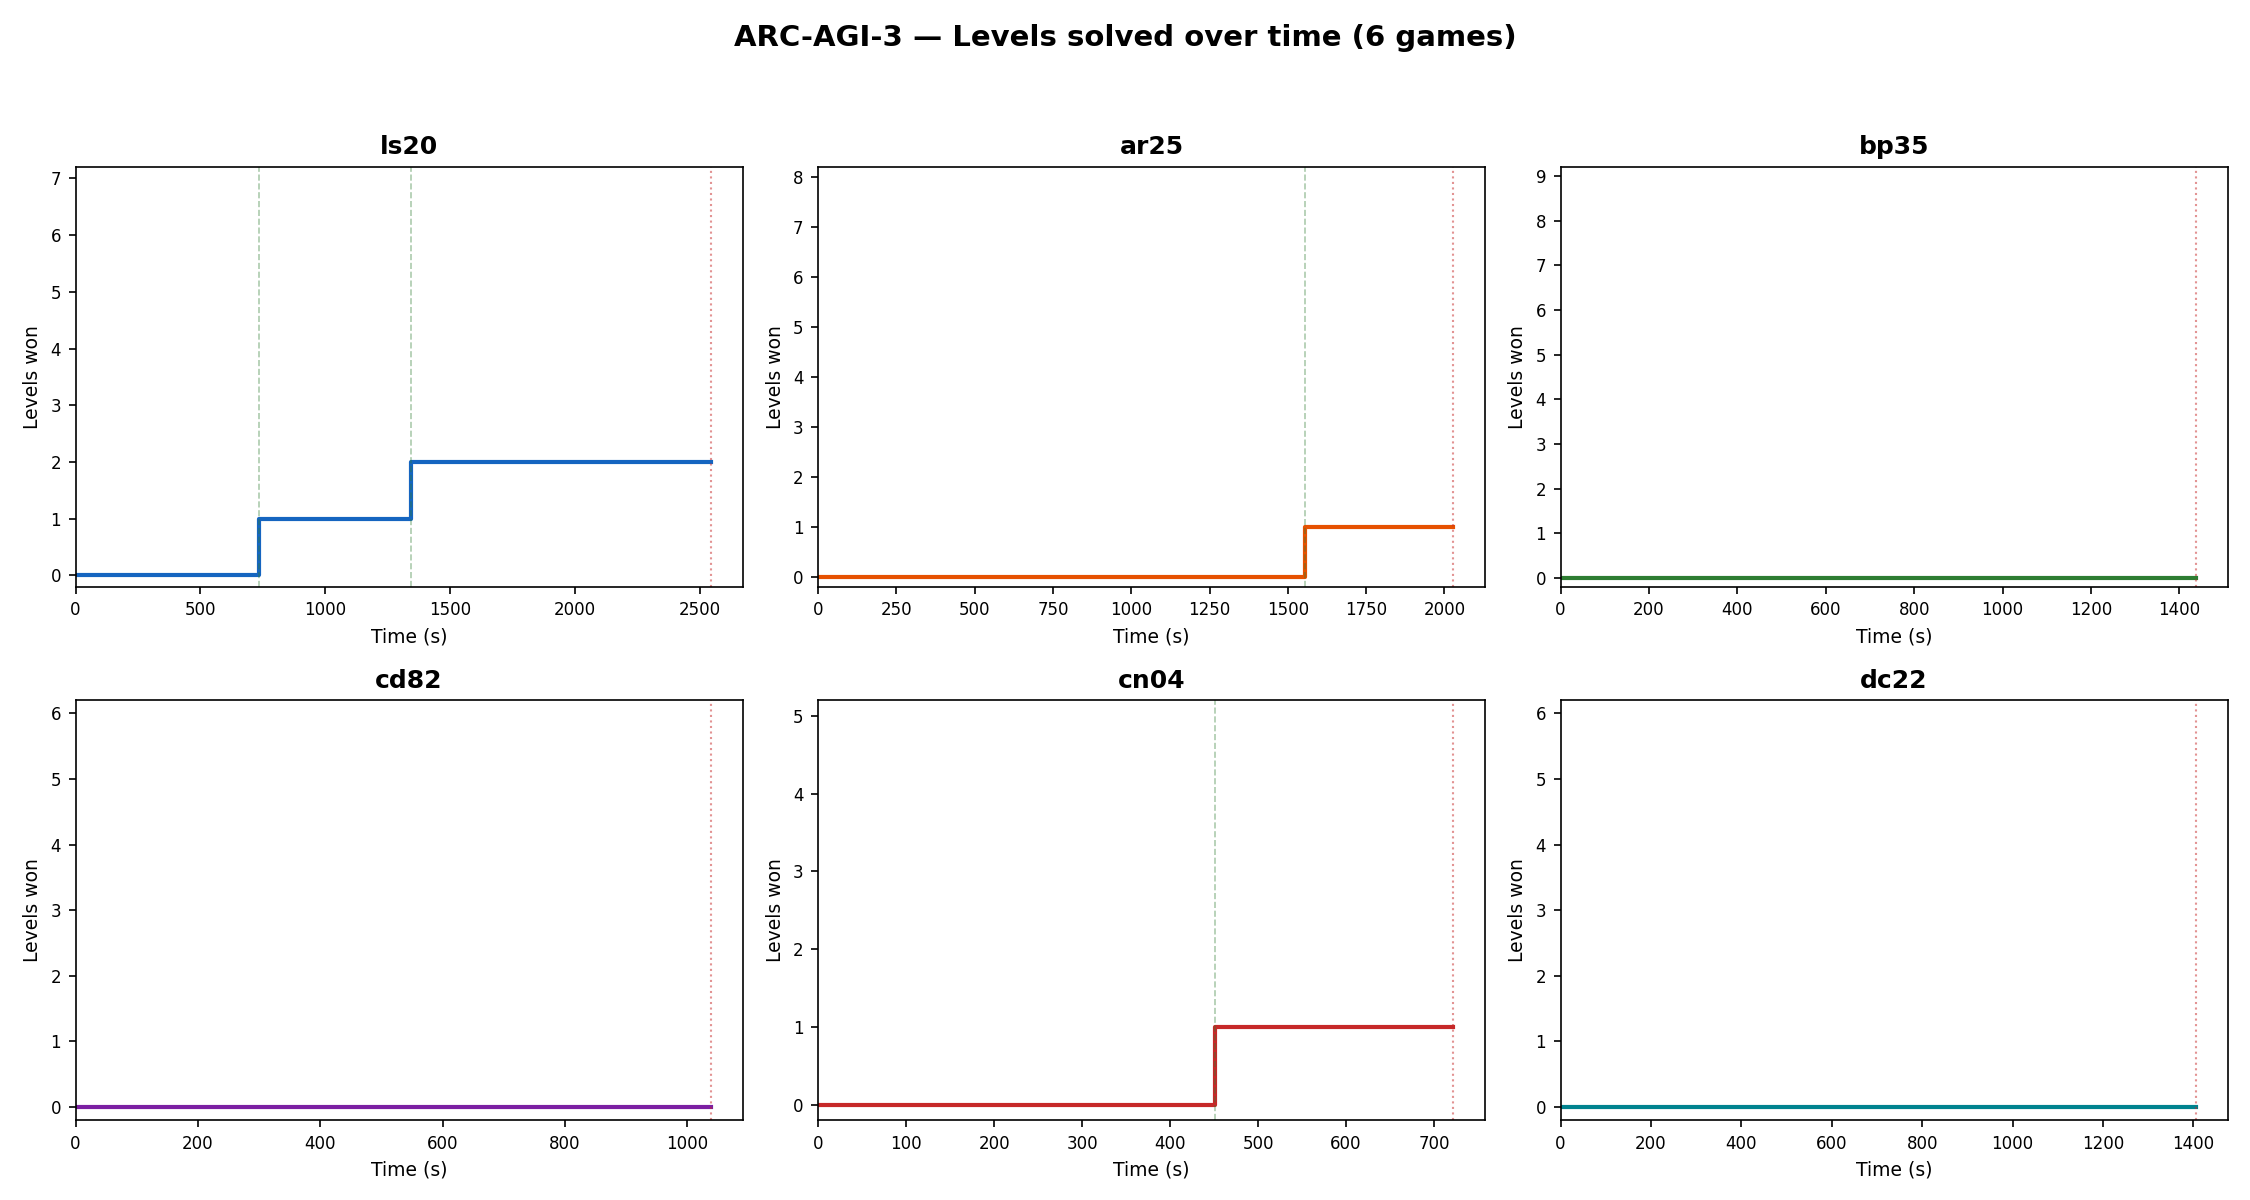
\includegraphics[width=\textwidth]{combined_plots/all_games_time.png}
\caption{Levels solved over wall-clock time for all 6 games. In the single-pass architecture, all reasoning time is concentrated in the analysis phase (one long flat segment); level execution is near-instantaneous.}
\label{fig:time}
\end{figure}

\begin{figure}[h]
\centering
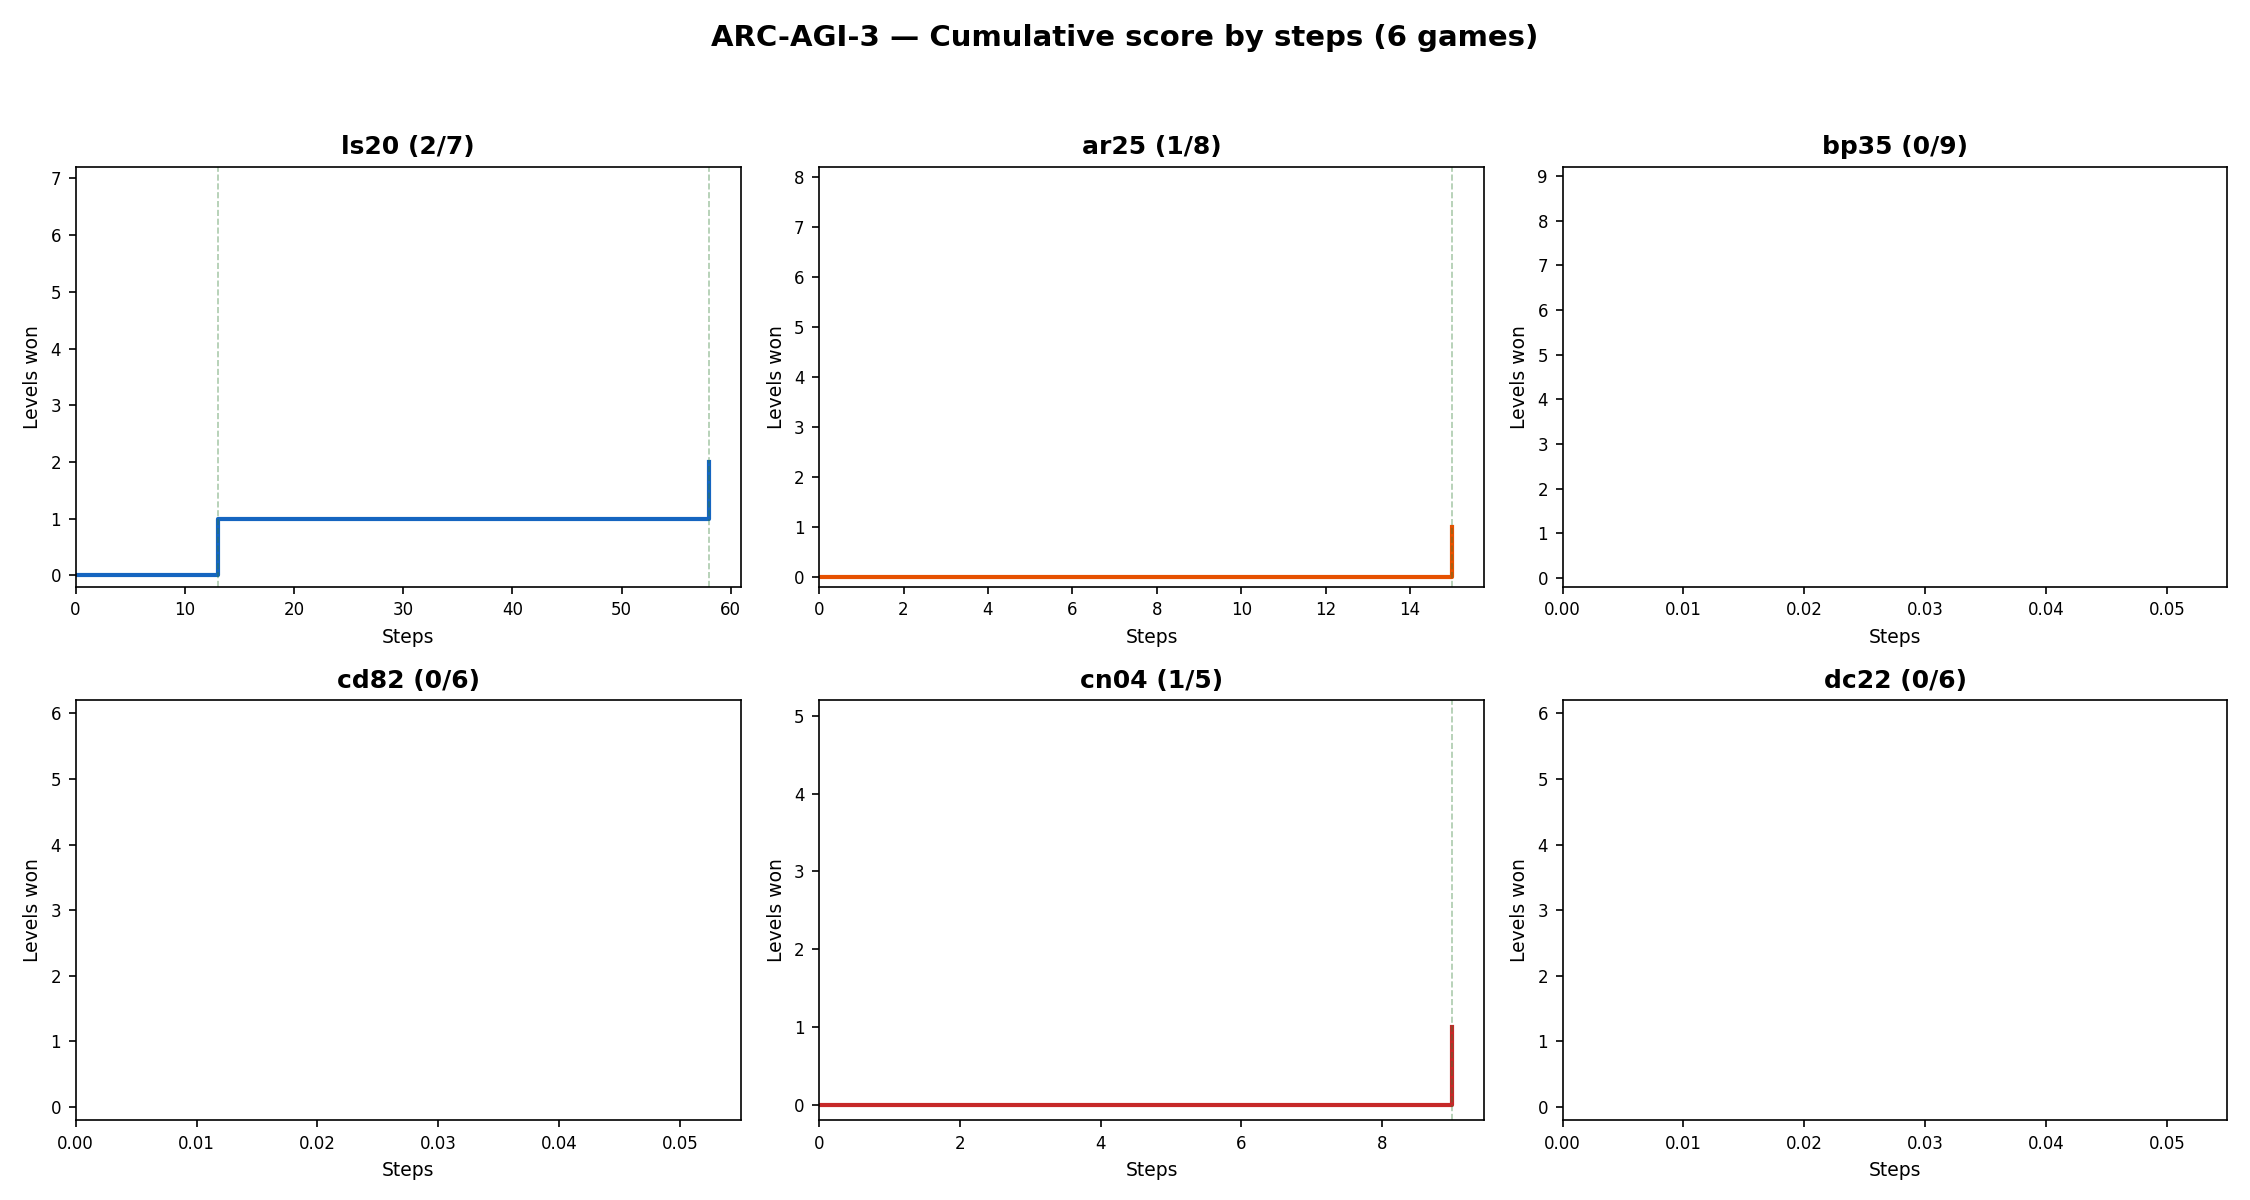
\includegraphics[width=\textwidth]{combined_plots/all_games_score.png}
\caption{Cumulative levels solved as a function of total steps (actions) executed. Subplot titles show final score. Games that failed on Level~1 (\texttt{bp35}, \texttt{dc22}) show zero cumulative steps since no moves were successfully executed.}
\label{fig:score}
\end{figure}

% ============================================================
\section{Discussion}

\subsection{Timing Analysis}
Analysis time varies widely across games (654.7--3600.1\,s), driven by source file complexity and the number of levels to solve in a single pass.
All four fully-solved games completed analysis in 654.7--2103.6\,s.
The two unsolved games (\texttt{bp35}, \texttt{dc22}) consumed 2700--3600\,s without producing parseable moves, suggesting they hit the limits of what can be reasoned about in a single pass.

\subsection{Failure Modes}
Two failure modes emerged among the 2 unsolved games:
\begin{enumerate}
  \item \textbf{Timeout / no moves} (1 case): \texttt{bp35} --- Claude Code exhausted the 3600\,s budget without producing parseable move sequences. The game has 9 levels with a restricted action space (\{3,4,6,7\}).
  \item \textbf{No moves parsed} (1 case): \texttt{dc22} --- Claude Code returned a response within 2700\,s but the harness could not extract valid move sequences. This may indicate the response did not follow the expected \texttt{```json} format, or the model failed to produce actionable solutions.
\end{enumerate}

The single-pass architecture exhibits an all-or-nothing dynamic: when reasoning succeeds, it produces complete solutions for every level; when it fails, no parseable output is generated at all.

\subsection{Cross-Game Observations}
\begin{itemize}
  \item 4 of 6 games were fully solved (26/41 levels, 63\%), a substantial improvement over the previous two-phase run (4/41 levels, 10\%).
  \item \texttt{cd82} required click coordinates for color selection and small basket firing, demonstrating that the \texttt{[6, x, y]} encoding works well for games with non-directional actions.
  \item \texttt{ls20} (7/7) succeeded in the later run after timing out in the earlier one, suggesting that results can be sensitive to run-to-run variance in reasoning.
  \item The two remaining unsolved games (\texttt{bp35}, \texttt{dc22}) may benefit from retry logic, increased timeouts, or a hybrid approach that falls back to per-level solving.
\end{itemize}

\end{document}
